\chapter{Materials and Methods}

This chapter focus on describing the used materials and methods utilized in this thesis. The acoustic emission tests (Section \ref{sec:AETest}) had 3 separate data acquisition systems, one using an industrial device (DISP-16C) made by Physical Acoustics (PAC), one with another industrial device (AMSY-5) made by Vallen Systems and a custom one denominated Streaming.

Both Streaming and Vallen data were analysed throughout the project duration, however, this thesis concentrates solely on the Streaming data. Both are similar in the way that they acquire temporal data from the AE (not its parameters), however, the AE waveforms captured by the Vallen system had several disadvantages when compared to the Streaming counterpart.

The Vallen data is a collection of fixed length AEs concatenated to form a $L \times N$ matrix where $L$ is the AE length and $N$ the number of captured AEs. This matrix was provided as a MATLAB formatted data file (.MAT) containing the waveform using 64-bit double-precision floating-point format. Unfortunately, this system is not guaranteed to capture all waveforms, this severely hinders some essential preprocessing stages (Sections \ref{sec:TOFDRemoval} and \ref{sec:bombRemoval}), making it a rather unreliable (the captured AE may not be from the crack propagation) and with no means of improving its reliability, therefore all of the Vallen data was discarded.

Thus, this chapter begins detailing the destructive test done, extends to the raw data format used, describes all the preprocessing done and the reasoning behind it, then details the waveform capture procedure all the way to creating the final dataset used to train a neural network model (Section \ref{sec:ann}) with parameters from both the AE temporal data and its frequency spectrum.


\section{Acoustic Emission Test} \label{sec:AETest}

The AE tests were performed by engineers of the Physical Metallurgy Laboratory (LAMEF) at the Federal University of Rio Grande do Sul (UFRGS). It uses a close-ended steel (API XL 60 series) pipe with $20$ inch diameter, $40$ metre length and $1.45$ centimetres of thickness, a semi-elliptical pre-crack extending until half of its thickness (approximately $0.7 cm$) was inserted at half its length.

%mention the rubber cape !!!!!!!!!!

The hydrostatic test consists of a gradual increase of pressure (after filling the tube) followed by plateaus until it bursts (Figure \ref{fig:pressure_time}). In total, $4$ (four) tests were done, with the first one discarded since it did not burst. They were denominated CP1, CP2, CP3 and CP4 respectively.

\begin{figure}[H]
	\centering
	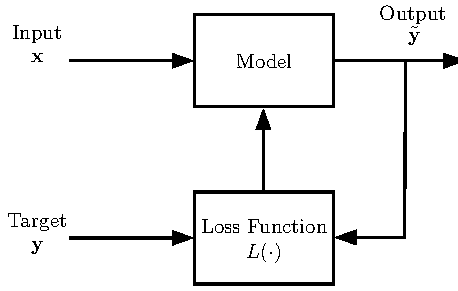
\includegraphics[width=0.1\textwidth]{sup_learning_schematic}
	\caption{Pressure and Crack Dimension for Test CPX}
	\label{fig:pressure_time}
\end{figure}

A sensor array was then disposed on top of the naked steel and the rubber cape (Figure \ref{fig:sensor_disposition}) throughout the tube's length. Immediately surrounding the crack a couple of ultrasound sensors were placed to measure its propagation throughout the test, those work based on Time-of-flight diffraction ultrasonics (TOFD) \cite{charlesworthEngineeringApplicationsUltrasonic2001}, \cite{silkPotentialScatteredDiffracted1975} and are named with respect to the technique (TOFD sensors).

% mention TOFD -> AE sensor or AE sensor -> TOFD ?

\begin{figure}[H]
	\centering
	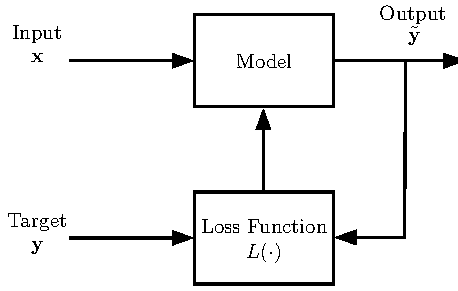
\includegraphics[width=0.1\textwidth]{sup_learning_schematic}
	\caption{Sensor Array Disposition for Test CP3}
	\label{fig:sensor_disposition}
\end{figure}

Three different streaming sensors (Figure \ref{fig:sensor_disposition}) were used, the R1.5 \cite{physicalacousticsR1520KHz}, R15\cite{physicalacousticsR15IAST150KHz} and WD \cite{physicalacousticsWD100900KHz} sensors. Their inner workings and configuration (including conditioning circuits) will not be discussed in this work. It is important to note however, that they work on different frequency ranges (Table \ref{tab:sensor_freq}) and naturally have diverse responses.

\begin{table}[H] \label{tab:sensor_freq}
	\centering
	\caption{Streaming Sensors Frequency Range.}
	\begin{tabular}{cc}
		\hline
		Sensor & Frequency Range (kHz) \\ \hline
		R1.5   & 5 - 20                \\
		R15    & 50 - 400              \\
		WD     & 100 - 900             \\ \hline
	\end{tabular}
\end{table}

These sensors were then sampled using a (not specified) 16 bit Analogue-to-Digital Converter (ADC) at $2.5 GHz$ during the whole test, their data was then put into a special formatted file created by National Instruments (NI), the Technical Data  Management Streaming (TDMS) file \cite{nationalinstrumentsNITDMSFile}. 


\section{Streaming Raw Data}

Normally, these files can be opened using some specific NI software like \textit{DIAdem} but the LAMEF engineers made slight modifications (Figure \ref{fig:lamef_mods}) when saving the ADC data, using a $32 bit$ word (normally holding one sample) made of two concatenated $16 bit$ integers (that came from the ADC), thus effectively doubling the amount of data stored without requiring additional space.

\begin{figure}[H]
	\centering
	\def\svgwidth{0.7\columnwidth}
	\input{images/low_level_mod_lamef_.pdf_tex}
	\caption{Low-Level Modifications Done to Signal Acquisition.}
	\label{fig:lamef_mods}
\end{figure}


In order to read the TDMS files, LAMEF provided a special compiled LABView routine that transforms each TDMS file to a binary one and a MATLAB script that loads the file to memory. Out of all the tests, only the first one (CP1) did not burst, even after $5$ filling cycles, since identifying the burst is essential (Section \ref{sec:objective}) all CP1 data was discarded and it will not be discussed any further.

A single TDMS file translates to roughly $6.7$ seconds (Figure \ref{fig:tdms_example}), containing $2^{24}$ samples taken from its $16$ different sensors (channels) leading to a $2^{24} \times 16$ integer (16-bit) matrix. In sum (Table \ref{tab:streaming_data}), all data came from (eventually) ruptured ducts and theoretically contain useful data.

\begin{table}[H]\label{tab:streaming_data}
	\centering
	\caption{Hydrostatic Test Summary}
	\resizebox{\columnwidth}{!}{%
	\begin{tabular}{ccccccc}
		\hline
		Test & Date       & \thead{Pre-Crack Depth\\ (millimetres)} & \thead{Rupture Cycle} & \thead{Pressure\\ at Rupture\\ (bar)} & \thead{Data Volume\\ (Gigabytes)}  & Files\\ \hline
		CP1  & 18/03/2015 & 5.5                           & X             & -                         & 3900    & X               \\
		CP2  & 28/07/2015 & 7.9                           & 1             & 230                       & 900     & 1513               \\
		CP3  & 06/11/2015 & 6.6                           & 1             & 264                       & 900 	& 1500                    \\
		CP4  & 23/05/2016 & 7.0                          & 2             & 283                       & 1500	&  4261                \\ \hline
	\end{tabular}%
}
\end{table}

\begin{figure}[H]
	\centering
	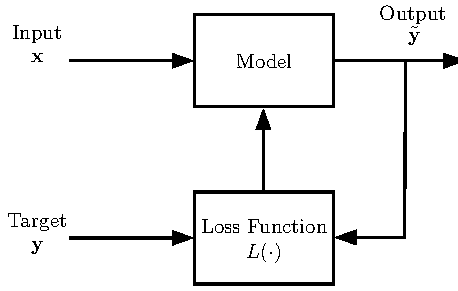
\includegraphics[width=0.1\textwidth]{sup_learning_schematic}
	\caption{Data from TDMS File 900, Channel 12 From Test CP3}
	\label{fig:tdms_example}
\end{figure}

\section{Preprocessing}
\subsection{Resolution Analysis}

\subsection{TOFD Removal} \label{sec:TOFDRemoval}
\subsection{Pressure Bomb Removal} \label{sec:bombRemoval}

\section{Wave Capture}
\subsection{Acoustic Emission Parameters}
\subsection{Frequency Data}

\section{Database Structure}

\section{Model Definition}

\subsection{Network Size}
\subsection{\textit{Transition Time Estimation}}
\subsection{Relevance Analysis}

